\documentclass{article}
\usepackage{icomp2026_conference,times}
\icompfinalcopy
\bibliographystyle{icomp2026_conference}
\usepackage[T1]{fontenc}
\usepackage{microtype,amsmath,amssymb,amsthm,booktabs,graphicx}
\usepackage[hidelinks]{hyperref}
\hypersetup{pdftitle={Exact Top-h Selection from Pivotal Votes: Integer Certification and Its Limits},pdfauthor={Anonymous authors}}
\newtheorem{theorem}{Theorem}
\newtheorem{proposition}[theorem]{Proposition}
\DeclareMathOperator{\sgn}{sgn}
\newcommand{\EE}{\mathbb E}
\newcommand{\PP}{\mathbb P}
\newcommand{\method}{pivotal minPI}
\title{Exact Top-$h$ Selection from Pivotal Votes:\\Integer Certification and Its Limits}
\author{Anonymous authors}
\begin{document}
\maketitle
\lhead{}
\renewcommand{\headrulewidth}{0pt}
\begin{abstract}
Pivotal minPI ranks features by the smallest mean signed contribution they make to a majority vote over specified peer counts. At a budget of $h$ features, a rounding error at the cutoff can change which columns are returned. On a gas-sensor matrix, two floating-point implementations selected the wrong member of a three-way tie. On a constructed matrix double precision missed the unique winner with a lead of $2.20\times10^{-21}$. We compute the prescribed top $h$ with two signed counts per row and peer count. Our direct selector prunes with one layer. When a common scale is safe, we compare signed machine-word sums directly. Otherwise we enclose the scores on a binary grid and resolve the cutoff with integer comparisons. Across 42 panels the median paired time ratios to unchecked floating-point pruning were 1.52, 1.51 and 1.59 at 2\%, 10\% and 50\% budgets, including ballot construction. On the 21 panels beyond the common-scale word bound, the ratios were 0.64, 0.57 and 0.56 to exact anchor pruning and 0.90, 0.91 and 0.90 to generating a floating-point proposal and checking its score and index bounds. On materials, doubling the sample used to construct the votes replaced all nine selected features even under exact scoring.

\end{abstract}
\noindent\textbf{Keywords}\quad voting games, exact arithmetic, feature selection, top-$h$ queries

\section{Introduction}
A sensor casts a positive vote when its reading is closer to a same-class reference than to a different-class one. Sensors on the same observation can disagree. Pivotal minPI credits each sensor with its signed change to the majority, averaged over peers at each specified group size. Its score is the smallest of these averages.

Votes of the same sign share a pivot count on each comparison. Since every layer bounds the minimum from above, a column whose bound falls below the cutoff needs no further layers. Rounding can replace a tied feature, as on the gas-sensor data, or erase a strict lead, as in our three-row example.

\paragraph{Related work}
Relief and its extensions score features from distances to same-class and different-class neighbours~\citep{kira1992relief,robnik2003relieff,sun2010local}. Model-utility games credit features for changes in prediction~\citep{cohen2007feature}. Earlier MinPI takes the minimum marginal contribution over individual coalitions in a thresholded utility game~\citep{shi2026minpi}. ShapG uses a feature-correlation graph to approximate Shapley values~\citep{zhao2025shapg}. In \method{}, the payoff is a majority on a single comparison, and each peer count defines a size-specific semivalue~\citep{dubey1981semivalues}.

Ternary bicooperative games allow players to join a supporting or opposing coalition~\citep{bilbao2010ternary}. In our game each row fixes the signs, and the participating subset varies. EPIC chooses among machine words, multiprecision integers and modular representations for weighted-game indices~\citep{staudacher2021power}. Threshold algorithms can retrieve a monotone aggregate from accessible attribute scores~\citep{fagin2003topk}. Here each such score requires a sum of signed counts. Their common layer denominator supplies the bounds for an interval filter with exact fallback~\citep{shewchuk1997adaptive}.

\section{The finite selection problem}
Let $V\in\{-1,0,1\}^{w\times p}$, with $w,p\ge1$. One row is one comparison, and a zero is an abstention. The payoff to an index set $S$ is
\begin{equation}
 U_r(S)=\sgn\!\left(\sum_{i\in S}v_{ri}\right), \qquad \sgn(0)=0 .\label{eq:game}
\end{equation}
For any nonempty $K\subseteq\{0,\ldots,p-1\}$ let $S_{jk}$ be a uniform $k$-subset of the peers of column $j$. Define
\begin{align}
 G_{kj}&=\frac1w\sum_{r=1}^{w}\EE\!\left[U_r(S_{jk}\cup\{j\})-U_r(S_{jk})\right],
 & T_j&=\min_{k\in K}G_{kj} .\label{eq:score}
\end{align}
Given $1\le h\le p$, return the $h$ columns with largest $T_j$, resolving ties in favour of the smaller original index. We return the selected indices in input order. The empty coalition gives $G_{0j}=w^{-1}\sum_r v_{rj}$, which we also use for comparisons when $0\notin K$.

If each retained feature has its own adverse peer count, the guaranteed total credit for a set $S$ is $\min_{(k_j)\in K^S}\sum_{j\in S}G_{k_j,j}=\sum_{j\in S}T_j$. The top $h$ maximize this sum. Under a single common adverse size the guarantee is $\min_{k\in K}\sum_{j\in S}G_{kj}$, which can be larger. Coalition payoff can differ from both guarantees. With all-positive votes a singleton wins every row, yet including a positive peer count in $K$ makes every $T_j$ zero.

\paragraph{Scope and choice of arithmetic}
The guarantee begins with $V$, its column order, $K$ and $h$. Sampling and floating-point neighbour search can change $V$. For layer denominators $D_k=\binom{p-1}{k}$, the direct selector computes $D=\mathrm{lcm}_{k\in K}D_k$ in arbitrary precision. If $wD\le 2^{63}-1$, signed machine words suffice on this common scale. Otherwise the direct selector bounds scores by integer intervals and resolves the boundary exactly. A second variant sums layers in machine words if $w\max_k D_k\le 2^{63}-1$, using arbitrary-precision cross products to compare fractions. Otherwise it uses the same interval path.

\section{Exact counting}
Remove the focal column from one row, leaving $a$ positive, $b$ negative and $c$ abstaining peers. Let $H_k(t)$ be the probability that a uniform $k$-subset has margin $t$. Cantor's generating function counts coalitions by size and weight after removing a player~\citep[Prop.~1]{bilbao2000power}. Here the number of subsets of size $k$ and margin $t$ is the coefficient of $x^kz^t$ in $(1+xz)^a(1+xz^{-1})^b(1+x)^c$. The sampled counts $(n_+,n_-,n_0)$ jointly follow a multivariate hypergeometric distribution. Columns of the same sign share a pivot count. This reduces each row to at most two counts per layer for certifying membership at the budget cutoff.

\begin{theorem}\label{thm:pivotal}
For $a+b+c=p-1$, $0\le k\le p-1$ and integer $t$, let $\mathcal C_{k,t}$ contain the nonnegative triples $(n_+,n_-,n_0)$ with sum $k$ and difference $n_+-n_-=t$. Then
\begin{equation}
 H_k(t)=\frac{1}{D_k}
 \sum_{(n_+,n_-,n_0)\in\mathcal C_{k,t}}
 \binom{a}{n_+}\binom{b}{n_-}\binom{c}{n_0}\,.\label{eq:mass}
\end{equation}
Assign each binomial coefficient the value zero outside its feasible range. The mean increment contributed by the focal coordinate on this row is
\begin{equation}
 \begin{cases}
  H_k(-1)+H_k(0), &v_{rj}=+1,\\
  -H_k(0)-H_k(1), &v_{rj}=-1,\\
  0, &v_{rj}=0.
 \end{cases}\label{eq:identity}
\end{equation}
\end{theorem}
\begin{proof}
Expanding the product counts each indexed subset of margin $t$ once, giving~\eqref{eq:mass} after normalization. A positive vote raises the payoff by one at margins $-1,0$, and a negative vote lowers it by one at margins $0,1$. At every other margin the focal sign leaves the payoff unchanged. An abstention always contributes zero.
\end{proof}

\paragraph{Sharing the counts}
All positive focal votes share $A_{rk}=H_k(-1)+H_k(0)$ computed after removing one positive vote. All negative focal votes share the magnitude $B_{rk}=H_k(0)+H_k(1)$ after removing one negative vote. Assign zero weight to an absent sign. Then
\begin{equation}
 G_{kj}=\frac1w\sum_r\bigl(A_{rk}\mathbf 1_{\{v_{rj}=1\}}-B_{rk}\mathbf 1_{\{v_{rj}=-1\}}\bigr)\,.\label{eq:weights}
\end{equation}
When a row contains no abstentions, the summand is $(A_{rk}+B_{rk})v_{rj}/2+(A_{rk}-B_{rk})/2$. The second term shifts all columns equally. On an abstention-free matrix, a weighted sum of the signed votes therefore determines the order at each $k$. Identical vote vectors tie.

Fixing $n_+-n_-=t$ leaves at most $\lfloor k/2\rfloor+1$ terms. Full floating-point scoring tabulates log binomials up to $k_{\max}=\max K$ and costs $O(p(k_{\max}+1)+w\sum_k(k+1)+|K|wp)$ before sorting. Lean~4 checks the subset counts, normalization and pointwise increments. Enumeration up to five peers matched all 1,358 margin counts and 798 signed numerators.

\subsection{Integer certificates for the selected support}
Choose an anchor $s\in K$. Its score $B_j=G_{sj}$ bounds $T_j$ from above. Evaluate the minima of the $h$ columns with the largest bounds and call this candidate set $C$.

\begin{proposition}\label{prop:screen}
Given an upper bound $U_i\ge T_i$ for each outsider and a lower bound $\ell\le\min_{j\in C}T_j$, discarding outsiders with $U_i<\ell$ preserves the top-$h$ support of~\eqref{eq:score} under the fixed tie order.
\end{proposition}
\begin{proof}
For each discarded $i$, $T_i\le U_i<\ell\le\min_{j\in C}T_j$, so all $h$ candidates outrank $i$. Equality leaves $i$ eligible.
\end{proof}
Exact anchor scores and candidate minima supply these bounds directly. Rounded scores require certified one-sided errors for the same comparison.
On the common scale each row contributes at most $D$ in magnitude. Every partial sum fits and can be negated safely when $wD\le2^{63}-1$. Above this sufficient bound the direct selector uses intervals with exact fallback~\citep{shewchuk1997adaptive}.

On row $r$ write $n_{rkj}/D_k$ for the signed pivot from~\eqref{eq:identity}, including zero for abstention. Choose $Q=2^b$. Compute the integer $f_{rkj}=\lfloor Qn_{rkj}/D_k\rfloor$ once per row and sign. For negative numerators the floor is towards $-\infty$. Let $E_k$ count rows on which either occurring sign has a nonzero remainder. With $L_{kj}=\sum_r f_{rkj}$,
\begin{equation}
 L_{kj}\ \le\ wQG_{kj}\ \le\ L_{kj}+E_k. \label{eq:grid}
\end{equation}
Each counted row loses less than one grid unit. Minimizing both endpoints over $k$ gives $L_j\le wQT_j\le U_j$ of width at most $w$. An all-abstaining column has zero numerators, so we tighten its enclosure to $[0,0]$ while keeping it in other columns' peer sets. The limit $0\le b\le62-\operatorname{bitlength}(w)$ leaves room for the sum and its error allowance. When 40 bits fit, the default normalized width is at most $2^{-40}$.

\begin{proposition}\label{prop:rational}
Start with any $h$ anchor candidates, refine all their intervals and discard outsiders whose anchor upper bound lies strictly below the smallest candidate lower bound. Refine the remaining intervals. Let $l,u$ be the $h$th largest remaining lower and upper endpoints. Include columns with $L_j>u$, exclude those with $U_j<l$, and fill the open places by exact scores among the rest. This returns the rational top-$h$ support with the prescribed tie order.
\end{proposition}
\begin{proof}
Each of the $h$ candidates scores strictly above every discarded upper bound. The $h$th largest true score in grid units belongs to $[l,u]$ by monotonicity of order statistics. The two strict tests therefore settle membership on either side. At the boundary compare the integers $\min_k (D/D_k)\sum_r n_{rkj}=wD T_j$. Their order, including equality, is exact.
\end{proof}
Write $\theta=T_{(h)}$ for the $h$th largest score. In score units each interval has width at most $\eta=\max_k E_k/(wQ)$, and both endpoint cutoffs lie within $\eta$ of $\theta$. Each undecided interval intersects the cutoff interval, putting its score in $[\theta-2\eta,\theta+2\eta]$. If $h<p$ and $T_{(h)}-T_{(h+1)}>2\eta$, this band contains only selected columns, which fill the open places. Since $\eta\le2^{-b}$, a true gap above $2^{1-b}$ suffices. The algorithm tests certified endpoints. Rounded gaps cannot establish this condition, and point intervals can settle ties. At $h=p$ membership is immediate.

\paragraph{Computational cost}
Group rows by tally and start at $\max K$. Take all undecided columns if they fill the open places. An all-point boundary is exact. On a mixed boundary reuse silent columns' zeros and rescore the other columns.

For $u$ distinct row compositions, a layer uses $O(u(k+1))$ products of binomial coefficients. At $p=16{,}384$, $D_{16}$ has 180 bits. After the $wp$ input scan and weight preparation, word accumulation costs $O(wp+(|K|-1)wc)$ for $c$ columns refined at secondary layers. For $m$ columns sent to exact scoring it adds $O(|K|wm)$ arbitrary-precision additions and $O(|K|m)$ scale multiplications. Sorting uses $O(p\log p)$ comparisons. Scaled scores need at most $1+\lceil\log_2(wD+1)\rceil$ signed bits, with linear bit cost for addition or comparison. Dense storage comprises the votes, $O(w|K|)$ row weights and $O(wp)$ candidate workspace.

At the original budget, 40 of 42 measured gaps exceeded $2^{-39}$, enough at 40 bits to avoid rescoring. The symmetric band contained just one column on 39 panels. On the additional positive-gap panel it included other selected columns tied at the cutoff. A tied maximum in Figure~\ref{fig:work}d required $m=2{,}048$ of 4,096 columns. Full fallback occurs even at $h=1$. Take $p=128$ and two rows, the first with 64 positive and 64 negative votes and the second its negative. For $K=\{0,4,16\}$ the rows cancel and all scores vanish. The 67-bit denominator $D_{16}=\binom{127}{16}$ puts the direct selector on its interval path. The nonzero pivot magnitudes at sizes 4 and 16 have odd reduced denominators greater than one. At every supported grid precision, flooring opposite pivots gives a sum of $-1$ and the two row allowances add two. Taking the minimum with the exact zero at layer~0 gives every column the same interval $[-1,0]$ in grid units. All 128 columns undergo screening and exact rescoring ($c=m=p$). Lean checks the signed floor and sum bounds, strict pruning and native sum safety.


\section{Algorithmic validation}
We fix the ballots, peer counts, budget and tie rule within each timing comparison. The default $h=\lceil p/10\rceil$ retains one feature in ten. The default layers compare an unaided vote with four and sixteen peers, capped at $p-1$ with duplicates removed. Grid precision affects the cost of certifying this target.

\subsection{Reproducing budget-boundary decisions}\label{sec:boundary}
\begin{figure}[t]
\centering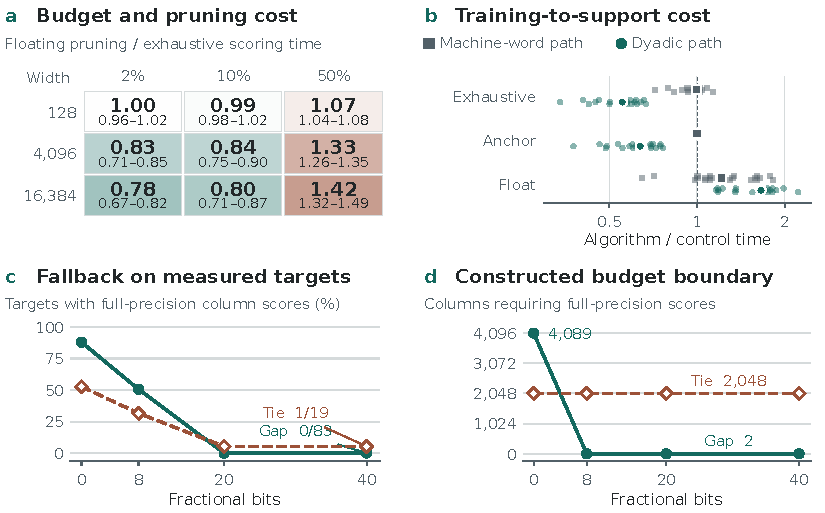
\includegraphics[width=\linewidth]{figures/cost-frontier.pdf}
\caption{(a) Floating pruning/exhaustive scoring time across 12 matrices per width and budget. Entries show medians and interquartile ranges. (b) Original 10\% training-to-support timings before tightening the bounds for silent columns. Pale marks show minPI/comparator ratios of five-call medians. Large marks give the median over 21 panels per path. (c) Fraction of targets requiring any full-precision score on six selected matrices. At 40 bits these counts are 0/83 positive gaps and 1/19 ties. (d) Number of individual columns rescored on two 4,096-column constructions at $K=\{0,4,16\}$ and $h=1$.}
\label{fig:work}
\end{figure}

Adding $k=1$ to $K=\{0,4,16\}$ on gas (seed 1129) replaced ten of 64 columns. Without abstentions and with $p>1$, a focal vote changes the one-peer payoff when their signs differ. Its mean increment is $(pv_{rj}-M_r)/[2(p-1)]$ at margin $M_r$. Averaging over rows gives $G_{1j}=p(G_{0j}-\bar G_0)/[2(p-1)]$ with $\bar G_0=p^{-1}\sum_iG_{0i}$. Layer~1 preserves the order of $G_0$ but can change which layer attains the minimum.
On this $256\times128$ matrix, the signed vote sums are 86 for each of zero-based columns 45, 57 and 115 and 12,058 for the whole matrix. Thus all three give $G_1=(128\cdot86-12058)/(2\cdot256\cdot127)=-525/32512$, also their exact minimum over the four layers. One final division of these integers gives identical binary64 values. The tie spans ranks 63--65, admitting 45 and 57. In both floating implementations, 57 and 115 took the places, exceeding 45 by 16 and 24 units in the last place, respectively. Floating pruning agreed with direct counts on the other 101 targets from six selected matrices. The package replays both selections from the archived votes.


For a strict winner take $p=4096$, $K=\{0,4,16\}$ and $h=1$. Number columns from zero. The first row votes positively on 0--2047 and the second on $\{0,1\}\cup\{2048,\ldots,4093\}$, with all other votes negative. They share two positives (0, 1) and two negatives (4094, 4095). The third row votes negatively on 0 and 4089--4095 and positively elsewhere. A size-16 peer tie for column 1 takes all eight negatives and eight positives. Column 0 has only seven negative peers. The resulting lead is
\[
 \Delta=\frac{\binom{4087}{8}}{3\binom{4095}{16}}
       =\frac{2}{908054843662451242401}\simeq 2.20\times10^{-21}.
\]
At size 16 the balanced rows give every other column a nonpositive sum by sign symmetry. The third row adds at most $\Delta$ to its mean. For columns 0 and 1,~\eqref{eq:mass} gives size-16 scores between 0.13117 and 0.13118. Their size-4 scores exceed 0.25 and their size-0 scores are $1/3$ and 1. Size 16 binds for both, so column 1 is the unique winner. The two exact minima lie approximately 0.484296 and 0.484375 ulp above the same binary64 value. Even a single final rounding to nearest therefore makes the index rule select column 0.

Over 32 paired calls on fixed ballots, median scoring times for direct certification and for the floating-point proposal with verification were 5.10 and 5.82\,ms on gas, and 0.273 and 0.633\,ms on the strict winner. Both methods rescored three gas columns and two constructed columns at full precision. Verification replaced 115 with 45 on gas and 0 with 1 on the construction.


\subsection{Cost at the selection boundary}\label{sec:frontier}
Three draws at each width (128, 4,096 or 16,384 columns), row count (32 or 192) and abstention rate (0 or 75\%) gave 36 matrices. At width 16,384 the median floating pruning/exhaustive ratios were 0.78, 0.80 and 1.42 at the three budgets (Figure~\ref{fig:work}a). The initial candidates sufficed on all 36 matrices at 10\% and only three at 50\%. An outside bound equalled the cutoff on two of the 108 targets.

\paragraph{Training-to-support timing protocol}
Each call rebuilt the votes for one budget. A stored exact ranking could serve several budgets. The 42 observed panels comprised five 75/25 splits per benchmark (breast cancer, digits, Spambase, ISOLET, Gisette, diabetes and Communities and Crime), three witness seeds on one split each for gas and materials, and one participant split for MHEALTH. Five more splits used the artificial Madelon benchmark~\citep{guyon2004challenge}. After one warm-up we compared five-call medians within panels. The quartiles in Table~\ref{tab:crossbudget} describe variation across panels, whose splits can share observations.

At the original budget, floating-point and integer scoring agreed on all 42 measured panels and all five artificial splits. Two measured panels had a cutoff tie. The smallest positive gap was $1.25\times10^{-6}$ (Gisette).

\paragraph{Selection time with machine-word arithmetic}
The dyadic path in the initial 10\% benchmark used row-wide error allowances (Table~\ref{tab:raw-cost}, Figure~\ref{fig:work}b). The median paired time ratio over all 42 panels was 1.36 against unchecked floating pruning, 0.88 against exact anchor pruning and 0.69 against exhaustive integer scoring.

The median fraction of columns requiring other layers was 38.5\% with $G_0$ as the anchor, 28.9\% with $G_4$ and 10.3\% with the largest layer. We chose the largest after observing its frequent agreement with the minimum in earlier runs.

We tested whether raising the exact anchor cutoff in Proposition~\ref{prop:screen} saves work. On fixed ballots we sorted upper keys $(G_{\max K,j},-j)$ and scored the first $h$ columns. After each further score we updated the weakest retained key and stopped once the next upper key fell below it. All three variants paid for the anchor and its sort. Compared with a frozen cutoff, updates saved columns on 2, 6 and 14 of 42 panels as the budget increased, from 3,161 to 2,515 on one half-width Gisette panel. Median time ratios to frozen scoring ranged from 0.999 to 1.002 with batched evaluation and 0.986 to 1.002 with one-column evaluation.

\begin{table}[!htbp]
\centering\small
\caption{Selection and downstream model times at the 10\% feature budget, in milliseconds.}
\label{tab:raw-cost}
\newcommand{\minpiTimingRows}{%
\multicolumn{7}{@{}l}{\itshape Machine-word range ($wD\le 2^{63}-1$), 21 panels}\\[1pt]
Diabetes & 1/10 & 2.54 & 2.81 & 2.61 & 2.61 & 1.62\\
Breast cancer & 3/30 & 2.42 & 2.52 & 2.53 & 2.53 & 2.34\\
MHEALTH & 4/40 & 14.77 & 14.41 & 14.53 & 14.53 & 28.82\\
Spambase & 6/57 & 3.73 & 6.31 & 5.10 & 5.10 & 2.85\\
Digits & 7/64 & 2.91 & 4.68 & 4.72 & 4.72 & 5.77\\
\addlinespace[4pt]
\multicolumn{7}{@{}l}{\itshape Above the machine-word range ($wD>2^{63}-1$), 21 panels}\\[1pt]
Materials & 9/81 & 4.52 & 12.05 & 11.44 & 7.92 & 5.94\\
Crime & 11/102 & 3.14 & 11.70 & 11.27 & 6.04 & 2.28\\
Gas & 13/128 & 4.36 & 10.79 & 9.84 & 5.91 & 11.82\\
ISOLET & 62/617 & 7.03 & 28.90 & 20.93 & 12.29 & 59.57\\
Gisette & 500/5,000 & 40.87 & 85.46 & 65.66 & 48.71 & 91.62
}

\setlength{\tabcolsep}{3pt}
\begin{tabular*}{\linewidth}{@{\extracolsep{\fill}}lrrrrrr@{}}
\toprule
 & & \multicolumn{1}{c}{Float} & \multicolumn{3}{c}{Exact selection} & \multicolumn{1}{c@{}}{Model}\\
\cmidrule(lr){3-3}\cmidrule(lr){4-6}\cmidrule(l){7-7}
Source & $h/p$ & Pruned & Exhaustive & Anchor & \textbf{minPI} & Fit + predict\\
\midrule
\minpiTimingRows\\
\bottomrule
\end{tabular*}
\par\smallskip
\begin{minipage}{\linewidth}\footnotesize
Entries are source medians of five-run panel medians. Selection includes ballot construction from training arrays (derived windows for MHEALTH). Model times include column extraction, fitting and prediction with standardized ridge or, for MHEALTH, logistic regression.
\end{minipage}
\end{table}

\paragraph{Cost of exact membership at three budgets}
Table~\ref{tab:crossbudget} times all five policies in the same run, rotating each through all five positions. The two smaller budgets both select one column on each diabetes split (126 budget entries, 121 distinct panel--width pairs). At 10\%, direct/unchecked was 1.51. Earlier runs with four policies gave 1.38 and 1.57 on the same panels. The initial row-wide implementation gave 1.36.

The verifier refines the proposal and every outsider whose anchor upper bound reaches its weakest lower bound. Strict separation accepted 41, 40 and 26 of 42 proposals at successive budgets. The index-aware test compares the worst selected key $(L_j,-j)$ with the best outside key $(U_i,-i)$. It accepted all 42 at each budget, resolving the 19 endpoint ties by index. Neither verifier needed full-precision column sums on those ties, and both corrected the two errors in Section~\ref{sec:boundary}. Including ballot construction and proposal generation, index-aware/strict median ratios were within 0.004 of one at all three budgets.

\begin{table}[t]\centering\small
\caption{Training-to-selection time ratios. Entries give the median [25th, 75th percentiles] of within-panel ratios of five-call medians (minPI/comparator). Fits denotes $wD\le2^{63}-1$, where exact anchor and minPI use the same kernel in separately timed calls. Both checks include generating the floating-point proposal.}
\label{tab:crossbudget}\setlength{\tabcolsep}{2pt}
\begin{tabular*}{\linewidth}{@{\extracolsep{\fill}}llrrr@{}}\toprule
Panels & Comparator & 2\% budget & 10\% budget & 50\% budget\\\midrule
All (42) & Pure float & 1.52 [1.16, 1.69] & 1.51 [1.13, 1.66] & 1.59 [1.16, 1.72] \\
\addlinespace[2pt]
Fits (21) & Pure float & 1.15 [1.07, 1.61] & 1.40 [1.08, 1.62] & 1.42 [1.09, 1.62] \\
 & Exact anchor & 1.00 [0.99, 1.03] & 1.00 [0.97, 1.00] & 1.00 [0.99, 1.01] \\
 & Float + strict check & 0.90 [0.86, 0.91] & 0.89 [0.82, 0.92] & 0.89 [0.85, 0.90] \\
 & Float + index check & 0.90 [0.86, 0.91] & 0.88 [0.86, 0.92] & 0.89 [0.85, 0.92] \\
\addlinespace[2pt]
Exceeds (21) & Pure float & 1.62 [1.32, 1.76] & 1.61 [1.20, 1.73] & 1.62 [1.34, 1.86] \\
 & Exact anchor & 0.64 [0.60, 0.69] & 0.57 [0.52, 0.68] & 0.56 [0.47, 0.59] \\
 & Float + strict check & 0.90 [0.89, 0.92] & 0.91 [0.87, 0.93] & 0.90 [0.86, 0.94] \\
 & Float + index check & 0.90 [0.86, 0.91] & 0.91 [0.89, 0.93] & 0.90 [0.87, 0.95] \\
\bottomrule\end{tabular*}
\end{table}

\paragraph{Layer scales}
Separate machine-word sums and arbitrary-precision cross products were feasible on 24 panels ($w\max_kD_k\le2^{63}-1$). On the three extra panels, all from one materials split, $w\max_kD_k=6.90\times10^{18}$, $wD=1.93\times10^{20}$ and cross products need 79--80 bits. Their median layer-wise/direct time ratios were 0.95, 0.95 and 0.96 from training arrays and 0.93, 0.90 and 0.94 on cached ballots. Across the 24 eligible panels the training ratios were 1.00, 0.99 and 1.00. Both routes used dyadic scoring on the other 18 and recovered all 126 reference supports.

For layer $k$, let $g_k$ be the gcd of $D_k$ and the signed pivot numerators actually present. Dividing both by $g_k$ preserves every row contribution. On the reduced common scale $D'=\mathrm{lcm}_{k\in K}(D_k/g_k)$ each summand has magnitude at most $D'$, so $wD'\le2^{63}-1$ suffices. Reduction added no panels to the 21 common-scale or 24 separate-layer cases. Probing the reduced common scale on the 21 raw overflows, including the gcd and lcm work before fallback, gave median training-to-support time ratios of 1.043, 1.021 and 1.043 to the direct selector.

\paragraph{Choosing the arithmetic}
For exact membership the direct selector uses the raw common scale when $wD\le2^{63}-1$ and certified intervals otherwise. Table~\ref{tab:crossbudget} charges both proposal methods for generating the list. With the ballots and list supplied, index-aware verification accepted all 126 proposals. Its median ratios to direct recomputation were 1.006, 1.002 and 0.995 at the three budgets, from five-call medians per panel. Verification sorts the supplied indices, and the direct dyadic path validates votes twice. For the wrong lists in Section~\ref{sec:boundary}, median correction/recomputation times over 32 pairs were 7.34/7.34\,ms on gas and 0.388/0.369\,ms on the strict winner.

For a predictive noninferiority claim, prespecify the deployment units, weights, loss tolerance and one-sided uncertainty bound. Fit paired models on the same training rows and assess loss on independent units. In the post hoc 64-column gas comparison, ridge trained on batches 1--7 gave exact minus floating-point balanced accuracies of $0$, $+0.081$ and $-0.045$ on batches 8--10. Using floating point cost 0.012 in mean balanced accuracy, within a tolerance of 0.02. Batch~9 exceeded it. Scoring alone in the Table~\ref{tab:crossbudget} calls gave median direct/unchecked ratios of 4.35, 3.87 and 4.24. Timings exclude model fitting.

\paragraph{Sensitivity to peer count, budget and precision}
The six observed matrices include the primary gas, materials and MHEALTH panels, two ties and the narrowest positive gap. Two constructions add a strict near tie and an exact tie. We tested each default layer, their minimum and the minima for $\{1,5,15\}$ and $\{0,1,4,16\}$ at budgets of one column, 10\% and 50\% (rounded up, duplicates removed). Peer counts on diabetes were capped at $p-1$. Adding size~1 changed one of 17 observed matrix--budget pairs.

Grid widths at $b=0,8,20,40$ range from one to about $10^{-12}$, with $2^{-20}$ near the narrowest original gap. Both interval implementations matched the integer reference in all 552 configurations. With point bounds for silent columns, 83, 48, 1 and 1 of the 102 observed targets required full-precision scoring (Figure~\ref{fig:work}c). At 40 bits the old allowance rescored 1,016 silent Gisette columns at half width for each of $K=\{4\},\{16\},\{1,5,15\}$. The tightened bounds left only three gas columns on one target in this deliberately selected sample. In panel d the strict winner has six distinct column vectors. Its 4,089 zero-bit fallback columns represent four vectors. Only columns 0 and 1 need rescoring at finer precisions. Copying row one onto row two gives the tied construction. At every precision columns 0--2047 (two of four vectors) need rescoring. Columns 1--2047 share the maximum and index 1 wins.


\section{Witness construction, support stability and prediction}
On benchmarks, gas and materials we cap the training sample at 256 to limit the $O(n_Qn_Rp)$ cost for $n_Q$ queries and $n_R$ disjoint references. Classification redistributes unfilled class quotas before splitting each class. Regression samples uniformly and groups by reference-response quintiles with distinct cut points.

We standardize each feature in single precision on the references, use one for standard deviations at or below $10^{-7}$, set missing standardized values to zero and clip at four standard deviations. From each feature's between-group to total variance ratio (zero for a constant) we subtract $(g-1)/\max(1,n_R-1)$ for $g$ groups and truncate at zero. Squared distances mix the normalized weights with 20\% uniform weight, or use uniform weights if all scores vanish.

For each query $q$, NumPy's \texttt{argpartition} retains the nearest four in each same- or other-group pool (all if fewer). We sort these by distance and reference-bank position. Ties across the partition lack a secondary key. Sorting whole pools by both keys changed two choices in 10,496 pools across 41 panels, leaving all votes intact. We pair the first hit and miss, then the last retained pair. Each pair casts $v_{rj}=\sgn(|q_j-m_j|-|q_j-h_j|)$, giving $w=2n_Q$ equally weighted rows. Fix the class allocation and reference bank $R$. If the queries are conditionally independent, their mean increments per query lie in $[-1,1]$ and Hoeffding's inequality gives
\[
 \Pr\{\max_j|T_j-T_j^*|\ge\epsilon\mid R\}\le2p|K|\exp(-n_Q\epsilon^2/2)
\]
by a union bound over columns and layers and the Lipschitz property of the minimum~\citep{hoeffding1963}. Here $T_j^*$ takes the minimum of the conditional expected layers. With $n_Q=128$, $p=5{,}000$ and $|K|=3$, a population cutoff gap above 0.912 suffices for 95\% recovery under this model. The five Gisette gaps ($1.3\times10^{-6}$ to $9.4\times10^{-5}$) came from finite tables sampled without replacement and do not establish this population condition.

\paragraph{Sensitivity to witness construction}
Certified and exhaustive scoring agreed on each of the 23 fixed matrices. Doubling the sample cap from 256 to 512 kept 158/500, 9/13 and 0/9 features on the first Gisette, gas and materials panels. Relative to the original supports, uniform neighbour weights gave Jaccard overlaps of 0.225, 0.857 and 0.286. Using the eighth neighbour instead of the fourth gave 0.495, 0.368 and 0.286. On materials, three and seven response bands both kept two of nine features. Over five training splits and five witness seeds per split, mean within-split Jaccard was 0.208 on Gisette and 0.194 on ISOLET (50 pairs each).

\subsection{When peer counts preserve the vote ordering}
Let $D_{rkj}$ denote the mean increment in~\eqref{eq:identity}. Define $\widetilde D_{rkj}$ as the expected increment when the $k$ indices are drawn independently from all $p$ columns, including $j$.

\begin{theorem}\label{thm:agreement}
For any ternary matrix and feasible $k$,
\begin{equation}
 |D_{rkj}-\widetilde D_{rkj}|
 \le 1-\prod_{s=1}^{k}\left(1-\frac{s}{p}\right)
 \le \min\left\{1,\frac{k(k+1)}{2p}\right\}.\label{eq:coupling}
\end{equation}
On a row without abstentions, let $q_r$ be the positive fraction. For even $k$,
\begin{equation}
 \widetilde D_{rkj}=v_{rj}\binom{k}{k/2}[q_r(1-q_r)]^{k/2}.\label{eq:kernel}
\end{equation}
The multiplier is one at $k=0$.
\end{theorem}
\begin{proof}
Conditioning on distinct draws that avoid $j$ gives a uniform peer subset. For fixed focal sign the increment ranges over an interval of length at most one, so conditioning changes its expectation by at most the probability of a focal hit or repeat. Counting valid ordered draws gives the product. A union bound over $k$ hits and $\binom{k}{2}$ pairs gives the second inequality. Without abstentions an even number of peers is pivotal only in a tie, which requires exactly $k/2$ positive draws.
\end{proof}
Without abstentions the exact tie probability at $k=2m$ is $\binom{a}{m}\binom{b}{m}/\binom{a+b}{2m}$. In the replacement approximation~\eqref{eq:kernel}, a 75\% positive row receives $0.5625$ times the balanced-row weight at $k=4$ and about $0.100$ at $k=16$. With abstentions, a sole positive voter among otherwise silent columns has marginal one at every size.

\begin{proposition}\label{prop:commonorder}
Suppose there are no abstentions. Set $a_{rk}=(A_{rk}+B_{rk})/2$ as in~\eqref{eq:weights}. For any $a_k>0$ write $e_k=w^{-1}\sum_r |a_{rk}-a_k|$. If
$G_{0j}-G_{0\ell}>2\max_{k\in K}(e_k/a_k)$, every specified layer and their minimum rank $j$ above $\ell$.
\end{proposition}
\begin{proof}
The row offsets in~\eqref{eq:weights} cancel upon subtraction. Thus
$G_{kj}-G_{k\ell}=a_k(G_{0j}-G_{0\ell})+
 w^{-1}\sum_r(a_{rk}-a_k)(v_{rj}-v_{r\ell})$.
The remainder has magnitude at most $2e_k$. Strict ordering at each of finitely many sizes gives strict ordering of the minima.
\end{proof}
For $h<p$, if the signed-mean gap at ranks $h,h+1$ exceeds this bound, all supports coincide. If the positive count is constant across rows and $A_k+B_k>0$ at each layer, all layers are strictly increasing affine functions of $G_0$ and preserve its ties.

For ternary ballots, write $D_{rk}(v)$ for the row increment of sign $v$. Take the range over signs present on that row. For $t_k>0$ define
\[
 B=\max_k w^{-1}\sum_r\operatorname{range}_{v}\{t_k D_{rk}(v)-v\}.
\]
The difference between any two row residuals is at most their range. Thus $G_{0j}-G_{0\ell}>B$ guarantees strict order in every layer and its minimum. If the $h$th signed mean exceeds an outsider's by more than $B$, that outsider can be discarded.

\paragraph{Coverage of the ordering bounds}
Only the three gas matrices among the 42 panels were free of abstentions (Proposition~\ref{prop:commonorder}). Abstentions comprised 0.039\% of MHEALTH votes and 6.02\% on the primary materials matrix. On gas we minimized $e_k/a_k$ by taking $1/a_k$ as a median of $1/a_{rk}$ weighted by $a_{rk}>0$. Rows with zero weight add a constant. The three thresholds, $1.309,1.345,1.299$, exceeded the respective signed-mean gaps of $0,0,0.03125$.

At the original budgets all layers agreed on seven of 42 supports. The minimum matched $G_0$ on 11 and the largest layer on 36. Full index-resolved rankings differed across layers on every matrix. The ternary bound excluded a median 501 of 5,000 Gisette columns and 159 of 617 ISOLET columns over five splits each. It excluded none elsewhere and certified no complete support.

\subsection{Instrument bias and sensor transfer}
In each of 48 simulated worlds we selected six of 60 channels: six stable (loadings 0.55--0.85), six reversing class effect on instrument two (1.30--1.70), and 48 background (1.50--2.50), all with independent standard Gaussian noise. Of 192 training comparisons, one third in expectation stayed on the query instrument and shared its background. Across instruments only one reference matched the background. We varied the probability that it was the hit ($1/2,2/3,5/6,1$). Logistic regression used 384 separate observations, two thirds from instrument two in expectation. We measured the lower instrument AUC on 1,536 fresh observations.

At the prespecified $5/6$ setting the mean lower AUC was 0.975 for the minimum, 0.567 for $G_0$ and 0.094 for $G_{16}$. The paired gain over $G_0$ was 0.408 (98.75\% world-bootstrap interval 0.346--0.460 for four primary contrasts). The strongest single layer in a post hoc comparison, $G_4$, scored 0.779. A univariate $F$ screen using the fitting labels scored 0.991. With fair matching, $G_0$ scored 0.990 and the minimum 0.977.

On MHEALTH, subjects 1--5 supplied training windows and 6--10 the prespecified holdout~\citep{banos2014mhealth}. Each of 192 wrist queries used its nearest hit and miss from other training subjects, resolving distance ties by increasing window index. For 128 queries the references came from the ankle and for 64 from the wrist. At $5/6$ the mean absolute size-16 marginal was 0.1820 within and 0.0009 across simulated instruments. The wrist--wrist and wrist--ankle means were 0.1140 and 0.1025, respectively. Among nonabstaining cross-instrument votes, the mean row fraction positive was 71.4\% under biased matching, 48.2\% under fair matching and 47.8\% on MHEALTH.

We measured alignment by the cross-device covariance of each channel's class means, weighting classes equally and dividing by the pooled within-device variance. Negative terms accounted for 67.1\% of total absolute covariance in the biased simulation and 2.2\% on MHEALTH (1.7--2.5\% in leave-one-training-subject-out calculations). Physical polarity and reference accuracy require separate measurements.

\begin{table}[!htbp]
\centering\small
\caption{Held-out prediction at the primary seed. Higher scores are better within each row.}
\label{tab:reliability}
\setlength{\tabcolsep}{3pt}
\begin{tabular*}{\linewidth}{@{\extracolsep{\fill}}llrrrrrrr@{}}
\toprule
 & & & \multicolumn{3}{c}{Voting scores} & \multicolumn{2}{c}{Other screens} & \\
\cmidrule(lr){4-6}\cmidrule(lr){7-8}
Source & Metric & $h/p$ & $G_0$ & \textbf{minPI} & $\Delta_0$ & $F$ & Random & Full width\\
\midrule
Gas & BA & 13/128 & 0.360 & 0.382 & $+0.022$ & 0.710 & 0.549 & 0.669\\
Materials & $R^2$ & 9/81 & 0.586 & 0.426 & $-0.160$ & 0.572 & 0.464 & 0.718\\
Wrist--ankle & BA & 4/40 & 0.463 & 0.421 & $-0.043$ & 0.323 & 0.474 & 0.705\\
\bottomrule
\end{tabular*}
\par\smallskip
\begin{minipage}{\linewidth}\footnotesize
Random uses one uniform $h$-subset drawn without replacement per task. $\Delta_0$ gives minPI minus $G_0$ before rounding. Gas balanced accuracy (BA) weights batches equally. Wrist--ankle BA averages each subject's lower location-specific BA.
\end{minipage}
\end{table}

\paragraph{Held-out prediction}
The minimum recovered the primary $G_{16}$ supports on gas, materials and MHEALTH, with respective inside--outside gaps of 0.0023, 0.0006 and 0.0037. With training and test rows fixed, 255, 241 and 130 of 256 further uniform supports outscored minPI on these tasks, respectively (Table~\ref{tab:reliability}). Gas ridge used batches 1--7 for training and 8--10 for testing~\citep{vergara2012gas}. The materials split kept duplicate descriptors and normalized compositions together, with 3,791 groups held out~\citep{hamidieh2018}. Materials ridge $R^2$ fell by 0.160 relative to $G_0$ (paired 95\% group-bootstrap interval $[-0.185,-0.136]$, fitted predictions fixed). With one of two further witness seeds, minPI replaced three $G_{16}$ columns. Relative to that $G_{16}$ support, test $R^2$ rose by 0.060 and $|S|^{-1}\sum_{j\in S}\min_k G_{kj}(V_{\rm test})$ fell by 0.0011. Both sets $S$ used the same $V_{\rm test}$, built from 128 queries and 128 disjoint references on the labelled prediction holdout. On wrist--ankle activity, four of five held-out subjects had lower BA with the minimum than with $G_0$. Across ten regression splits, tree MAE was unchanged on five and rose on five. Tree $R^2$ improved once, on a Crime split where MAE rose by 5.82.


\section{Discussion}
The certificate returns the prescribed support, including at a tied cutoff. Separated intervals can eliminate full-precision scoring. When $c=m=p$ the implementation pays for both screening and full scoring, even at $h=1$. The opposite rows cancel in this example. Reducing its fractions gives $wD'=632{,}667{,}422{,}750$ (40 bits), which permits machine-word sums directly. At $h=1$ the reduced selector took 0.189\,ms versus 0.316\,ms for the direct selector (32 paired calls on fixed votes). For the strict winner in Figure~\ref{fig:work}d the reduced bound still takes 119 bits. Identical columns there can share a computation if peer counts retain their multiplicities.

If every row has absolute margin at least two, removing one vote preserves the majority. Including size $p-1$ then gives $T_j\le0$ for every column. Proposition~\ref{prop:commonorder} can certify the support from the raw vote order. Its gap condition failed on all three eligible matrices, which still admit exact selection by~\eqref{eq:score}. Even under exact scoring, doubling the materials sample displaced all nine selected features.

In the biased simulation, size 16 gave cross-instrument comparisons almost no weight and favoured strong within-instrument features even when their polarity reversed. Raw signs favoured background features because hits often shared the query background. Each block scored poorly in one layer. Wrist and ankle comparisons had similar within- and cross-location pivotal weights. All four features selected at size 16 had positive cross-location covariance of their class means. Gas and materials lacked paired instruments for this comparison. With the same model fit and random seed, identical supports give identical predictions. The minimum and largest layer differed on six of 42 panels at the original budget and agreed on all three primary real-data panels. Estimating an average gain on new sources requires both the frequency of changed supports and their mean paired gain on independent observations.

\paragraph{Data and code availability}
The package contains data or reconstruction instructions, splits, supports, predictions, timings, proofs and code. We used NumPy, SciPy and scikit-learn~\citep{pedregosa2011sklearn}, with one numerical-library thread on an Intel Core Ultra~9 275HX under Windows~11.

\paragraph{Declaration of generative AI use}
OpenAI Codex assisted with research design, selector and experiment implementation, Lean formalization, data analysis, and manuscript drafting and revision.

\begingroup\raggedright
\bibliography{references}
\endgroup
\end{document}
